\documentclass[11pt]{article}
\usepackage{graphicx}
\title{Erlang NetInf NRS Initial Design Draft}
\author{Project CS 2012 - Backend}
\date{}
\DeclareGraphicsExtensions{.pdf,.png,.jpg}

\begin{document}

\maketitle

\section*{Introduction}
This document outlines an abstract design for an Erlang implementation of a NetInf NRS node. In this design we assume that the system runs on top of an HTTP Architecture, however it should be a fairly simple matter to change the underlying network topology.

\section*{Overall design}

The architecture of the NRS system consists of different processes and modules which interact with each other. There are two distinct process types, persistant and non persistant. The persistant processes will run for the entire uptime of the system whereas the lifetime of a non persistant process is the duration of its given task.

\subsection*{Layers}
The system architecture is divided into three distinct layers a network layer (http), convergence layer and an internal Erlang NetInf layer.   

\subsection*{Process hierarchy}
All persistant processes will be supervised by a root supervisor that is responsible for restarting them in case they should crash. Another supervisor will be responsible for the non persistant processes. 

\subsection*{Modules}
Each process in every layer of the architecture will have a corresponding module that defines its behaviour. There will also be additional modules that provide functionality not necessarily exclusive for a specific process. 

\begin{figure}[htb]
\centering
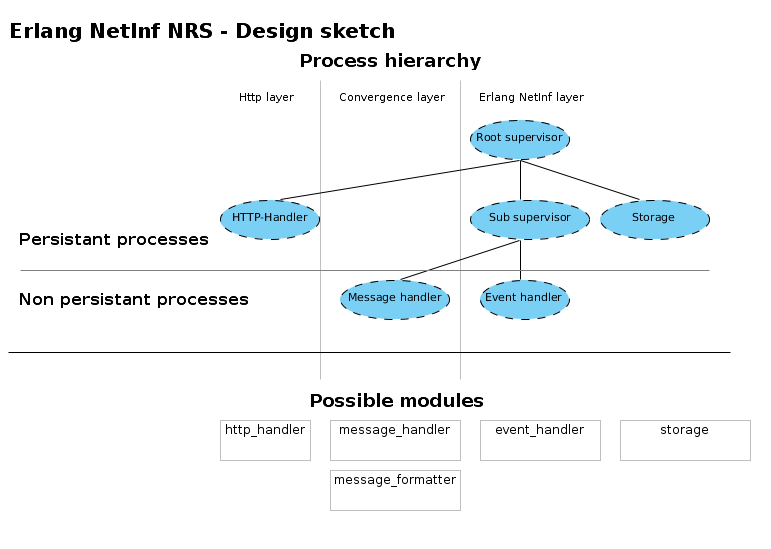
\includegraphics[width=1\textwidth]{pharch}
\caption{Three tier architecture of Erlang NetInf NRS node. The image shows the proposed process hierarchy and modules.}
\label{fig:architecture}
\end{figure}

\section*{Message flow}
Below are some diagrams that show the flow of messages between processes for get and publish requests and for a case when an error message would be generated.

\begin{figure}[htb]
\centering
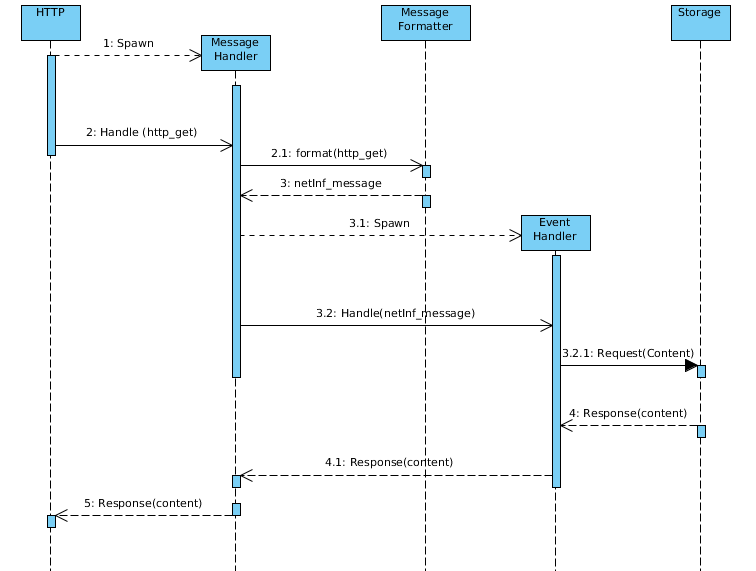
\includegraphics[width=1\textwidth]{seq_get}
\caption{Flow of information for a get request.}
\label{fig:sequence_get}
\end{figure}

\begin{figure}[htb]
\centering
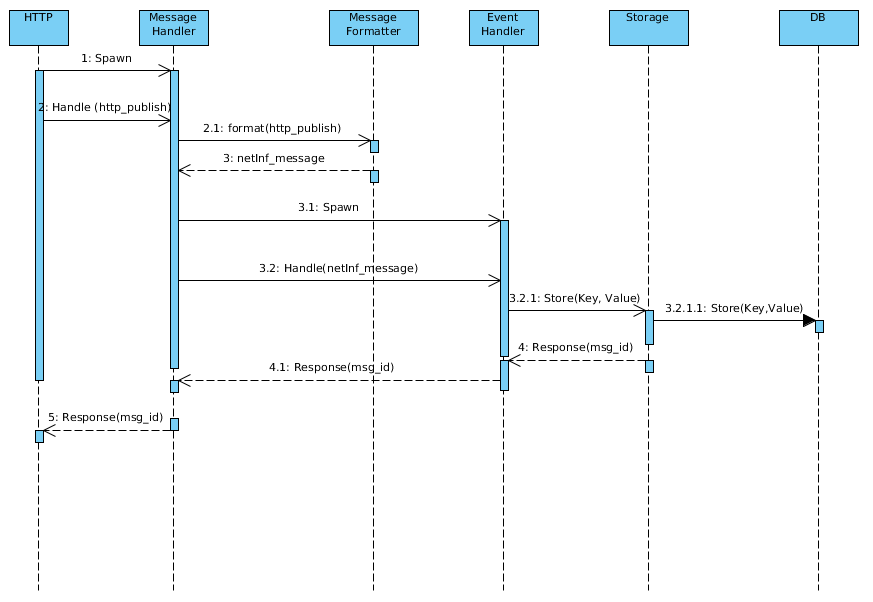
\includegraphics[width=1\textwidth]{seq_pub}
\caption{Flow of information for a publish request.}
\label{fig:sequence_pub}
\end{figure}

\begin{figure}[htb]
\centering
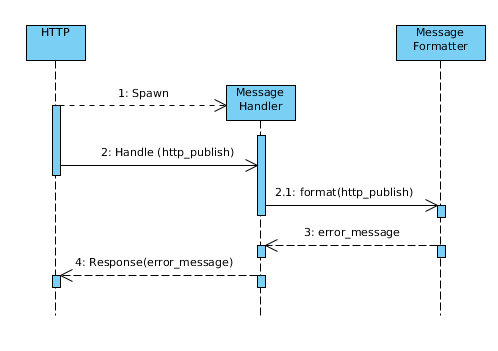
\includegraphics[width=1\textwidth]{seq_error}
\caption{Flow of information when receiving an erronous request.}
\label{fig:sequence_error}
\end{figure}


\end{document}